\documentclass[a4paper]{article}

\usepackage[english]{babel}
\usepackage{natbib}
\usepackage{amsmath,amsthm}
\usepackage{fancyvrb,listings,tikz,url}

\theoremstyle{definition}
\newtheorem{example}{Example}

\DefineVerbatimEnvironment{cmdsession}{Verbatim}{}

\lstnewenvironment{code}{\lstset{language=Haskell,basicstyle=\small,frame=trbl}}{}
\lstnewenvironment{spec}{\lstset{language=Haskell,basicstyle=\small,frame=TB}}{}

\setlength{\parindent}{0 ex}
\setlength{\parskip}{1 ex}

\newcommand{\bigO}{\mathcal{O}}
\newcommand{\cmd}[1]{\Verb@#1@}
\newcommand{\ignore}[1]{}  % Also used to fix syntax-highlighting
\newcommand{\ShFa}{Shannon--Fano}
\newcommand{\strategy}[1]{\marginpar{\bigskip\cmd{#1}}}


\title{An Information Theoretic Analysis of One-Step-Ahead Mastermind Strategies}
\author{Jouke Witteveen \and Jan van Eijck}


\begin{document}
\maketitle


\begin{abstract}
\noindent
This paper compares various one-step-ahead Mastermind strategies, rephrases some of these strategies in information-theoretic terms, and presents an improved strategy.
The paper gives documented Haskell code of all strategies that are discussed, and of their analysis.
Our code computes the full analysis of each strategy in a matter of seconds.
\end{abstract}


\section*{Introduction}

Mastermind is a knowledge update game that was invented in 1970, by Mordecai Meirowitz, and commercialized by Invicta Toys and Games (see \url{http://dspace.dial.pipex.com/town/road/gbd76/toys.htm}.
Mastermind is usually presented as a two-player game (zero sum, with imperfect information) between a code-maker and a code-breaker, but because the code-maker faces a computationally trivial task it makes sense to study it as a solitaire game for the code-breaker.
That Mastermind is a non-trivial game is witnessed by the fact that generalized Mastermind (played with two colours and $n$ pegs) is NP complete \citep{Bondt2004:npcomm}.

Solitary Mastermind fits the class of key-guessing games where the player figures out a designated element (the \emph{key}) of a set (the \emph{code space}) based on the information provided by the structured feedback to repeated guesses.
The aim of these games is to minimize the expected number of guesses needed to find the key.
In Mastermind, the key is assumed to be picked at random from the code space, under the uniform distribution.

\begin{example}
\label{ex:binary}
We can visualize strategies for key-guessing games as trees.
Suppose the set of possible keys is $\{1, 2, 3, 4, 5, 6\}$ and the feedback we get for a guess is whether the guess is equal to, greater than ($>$), or less than ($<$) the key.
Now, given a set of possible keys that are consistent with the feedback history, we choose a guess.
These choices, \texttt{<consistent set> $\to$ <guess>}, can be placed as nodes on a tree, where the edges are induced by the possible feedback to the guess.
For a certain procedure to determine our choices (a strategy) we can get a tree as in Figure~\ref{fig:binary}.
It is easy to see that this strategy is optimal for this particular game.

\begin{figure}
\begin{center}
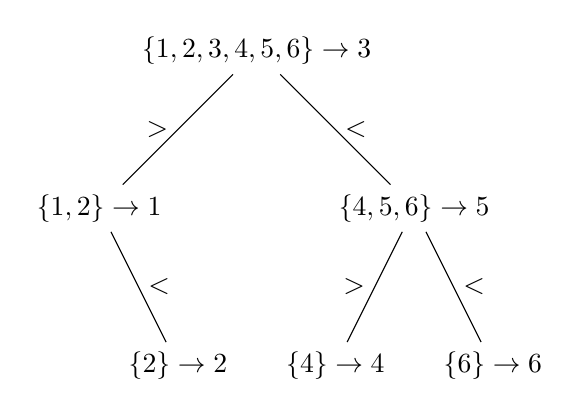
\begin{tikzpicture}[level/.style={sibling distance=40mm/#1},level distance=20mm]
  \node{$\{1, 2, 3, 4, 5, 6\} \to 3$}
    child{
      node{$\{1, 2\} \to 1$}
      child[missing]{}
      child{
        node{$\{2\} \to 2$}
        edge from parent node[right]{$<$}
      }
      edge from parent node[left]{$>$}
    }
    child{
      node{$\{4, 5, 6\} \to 5$}
      child{
        node{$\{4\} \to 4$}
        edge from parent node[left]{$>$}
      }
      child{
        node{$\{6\} \to 6$}
        edge from parent node[right]{$<$}
      }
      edge from parent node[right]{$<$}
    }
  ;
\end{tikzpicture}
\end{center}
\caption{
  A possible strategy for a key-guessing game on the set $\{1, 2, 3, 4, 5, 6\}$, with ordinary comparison as feedback.
  Every path in the tree corresponds to a play of the game.
}
\label{fig:binary}
\end{figure}
\end{example}

The Mastermind code space consists of all fixed length sequences of \emph{pegs} coloured from a palette.
Usually, the length of the sequences is four and the palette contains six colours.
The resulting code space of $6^4 = 1296$ codes will be our reference code space throughout this report.

Feedback in Mastermind consists of pairs $(b, w)$, where $b$ is the number of positions where the colour of the peg in the guessed code matches that of the peg in the key, and $w$ is the number of coloured pegs of the key that are in the wrong position in the guess.
E.g., if the key is $(\text{blue}, \text{green}, \text{blue}, \text{red})$, then the guess $(\text{green}, \text{yellow}, \text{red}, \text{red})$ will solicit feedback $(1, 2)$.

With each guess, the subset of the code space consistent with the guessing history decreases, hence our knowledge about the key increases.
It is known that the optimal strategy for Mastermind takes $4.340$ guesses on average to guess the key.
This result was found using exhaustive search \citep{KoyomaLai1993:aoms} and verified by \citet{Ville2013:aoms}.
In this report we will focus on \emph{one-step-ahead} strategies that consider only the possible outcomes of the next guess.


\section*{Implementation: The Mastermind Framework}

We present our code in literate programming style \citep{Knuth1992:lp}, in Haskell \citep{Haskell:www}.
If the module is loaded as object code in the GHC interpreter (\cmd{ghci -fobject-code Mastermind}), then the \cmd{summary} function defined in the Results section will compute its output in a matter of seconds.

\begin{code}
module Mastermind where
import Data.List
import qualified Data.Map as M
\end{code}

We will treat the palette as an alphabet.
Using letters instead of colours, we get the following datatype synonyms for codes and feedback:

\begin{code}
type Code        = String
type Feedback    = (Int, Int)
\end{code}

The most general definition of a strategy is that of a mapping of a subset of the code space, embodying all knowledge about a key at some point, to a code that will be the guess.
If the guess is part of the set of consistent (with the feedback history) codes, we say that the guess is \emph{consistent}, otherwise we call it \emph{inconsistent}.

\begin{code}
type Strategy    = [Code] -> Code
\end{code}

A more subtle kind of strategy rates all possible feedback outcomes of the next guess and picks the next guess on the basis of these ratings.
Because only the outcomes of the next guess are considered, these strategies can rightfully be called \emph{one-step-ahead} strategies.

\begin{code}
type Strategy1 a = Count (Counts Feedback) -> a
type Count a     = (a, Int)
type Counts a    = M.Map a Int
\end{code}

Generalized Mastermind code spaces can be generated from their alphabet and the number of pegs:

\begin{code}
mastermind :: [Char] -> Int -> [Code]
mastermind _       0    = [""]
mastermind colours pegs = [c:cs |
  c  <- colours,
  cs <- mastermind colours (pegs - 1)]
\end{code}

The usual game uses six colours and four pegs:

\begin{code}
theGame = mastermind ['A' .. 'F'] 4
\end{code}

The feedback to a guess, generated by a key:

\begin{code}
feedback :: Code -> Code -> Feedback
feedback guess key = (black, white)
  where black = length $ filter (uncurry (==)) $ zip guess key
        white = occursCount key guess - black

occursCount :: Code -> Code -> Int
occursCount _   []     = 0
occursCount key (x:xs)
  | x `elem` key       = 1 + occursCount (delete x key) xs
  | otherwise          = occursCount key xs
\end{code}

We will need an auxiliary function for partitioning based on a classifying function:

\begin{code}
partitionBy :: Ord b => (a -> b) -> [a] -> M.Map b [a]
partitionBy f xs = M.fromListWith (flip (++))
  [(f x, [x]) | x <- xs]
\end{code}

Example use of this function:
\begin{cmdsession}
GHCi> partitionBy (`mod` 3) [1 .. 10]
fromList [(0,[3,6,9]),(1,[1,4,7,10]),(2,[2,5,8])]
\end{cmdsession}


\section*{Strategies}

\subsection*{Elementary Strategies}
In our deterministic, stateless framework, arguably the simplest strategy is the naive strategy \citep{Shapiro1983:pml}.
This strategy selects the first consistent code as a guess:
\strategy{naivePlay}

\begin{code}
naivePlay :: Strategy
naivePlay = head
\end{code}

Observe that the naive strategy has time and space complexity $\bigO(1)$ and is thus very much a \emph{zero-steps-ahead} strategy.
Nevertheless, for some key-guessing games this strategy is optimal.
In particular it is optimal for searching the index of a designated element in an unordered array.
In this game, the index set forms the code space and the feedback is one of $\{\ne, =\}$.

For our analysis of one-step-ahead strategies, it is instructive to look at how a one-step-ahead strategy is transformed into a general strategy.
We realize such a transformation as follows:
\begin{enumerate}
\item
  Generate profiles of all possible feedback for all candidate guesses;
\item
  Partition the candidate guesses according to their feedback profile;
\item\label{strategy1:select}
  Run the one-step-ahead strategy on all feedback profiles and select the (union of the) set(s) of candidate guesses that minimizes the value assigned by the one-step-ahead strategy;
\item
  Pick the first consistent code from this set, or the first inconsistent code if there are no consistent codes in it.
\end{enumerate}

In our implementation, at step~\ref{strategy1:select}, we only take the first code from each set into consideration, as the other codes will be discarded in the next step anyway.
This is because either all codes from a partition cell are consistent (if the feedback indicating success is part of the feedback profile), or they are all inconsistent (otherwise).

Furthermore, we make the set of candidate guesses into a parameter, which defaults to the set of consistent guesses when empty.

\begin{code}
strategy1 :: Ord a => [Code] -> Strategy1 a -> Strategy
strategy1 candidates strat cons =
  minimum $ if null cs then is else cs
  where
    (cs, is) = partition (`elem` cons) $ bestCodes ratings
    ratings  = M.foldrWithKey acc [] $ partitionBy fbs from
    acc f xs = (:) ((strat (f, length xs)), [head xs])
    fbs x    = M.fromListWith (+)
                 [(feedback x k, 1) | k <- cons]
    from     = if null candidates then cons else candidates

bestCodes :: Ord a => [(a, [Code])] -> [Code]
bestCodes [(_, xs)]  = xs
bestCodes (xs:ys:zs) = case compare (fst xs) (fst ys) of
  LT -> bestCodes (xs:zs)
  GT -> bestCodes (ys:zs)
  EQ -> bestCodes ((fst xs, snd xs ++ snd ys):zs)
\end{code}

\ignore{$}
Observe that if \cmd{profile} is the feedback profile for a class of guesses, then \cmd{(M.elems . fst) profile} is a list of sizes of the consistent sets one step ahead.
Relating to Example~\ref{ex:binary}, it is a list of the sizes of the consistent sets in the children of a node.
If we are unlucky in a game, we end up with the largest of the possible resulting sets of consistent codes after a guess.
As we have to reduce the size of the set of consistent codes to $1$, eventually, this can be considered a \emph{worst case scenario}.
Minimizing this maximum size is suggested in \citep{Knuth1976:tcam} and can be taken as a strategy to minimize the maximum number of guesses needed.
\strategy{wcPlay}

\begin{code}
wcPlay :: Strategy1 Int
wcPlay = maximum . M.elems . fst
\end{code}

As we will see in the section on results, this approach indeed gives an optimal worst case scenario, on the condition that inconsistent guesses are allowed (the strategy would be expressed as \cmd{strategy1 theGame wcPlay}).
When applied to the game of Example~\ref{ex:binary}, this strategy would yield the optimal strategy displayed in Figure~\ref{fig:binary}.

\subsection*{Information Theory}
While \cmd{wcPlay} manages to minimize the maximum number of guesses needed, our goal is to minimize the expected number of guesses needed.
More visually, considering the tree corresponding to a strategy as was done in Example~\ref{ex:binary}, \cmd{wcPlay} minimizes the height of such a tree, whereas we would like to minimize the expected depth of the nodes that represent consistent guesses in such a tree.
In turn, this can be interpreted as an optimality criterion for a kind of encodings of the code space.

As shown in Figure~\ref{fig:binary}, the branches of the tree corresponding to a strategy are related to feedback values.
Thinking of all possible feedback values as the \emph{feedback alphabet}, a strategy thus induces an encoding of the code space with the feedback alphabet.
In this setting \citep{CoverThomas1991:eit}, the tree corresponding to the strategy is known as the encoding tree.

\begin{example}
\label{ex:encoding}
In the strategy depicted in Figure~\ref{fig:binary}, the code `$1$' would be encoded as `$>$', the code `$2$' would be encoded as `$><$', the code `$3$' would be encoded as `' (the empty string), and so on.
\end{example}

Now that we have seen that goodness of Mastermind strategies is equivalent to optimality of a kind of encodings, we might want to apply Huffman coding to the code space.
However, Huffman coding works in a bottom-up fashion, so applying it requires knowing which subsets of the code space constitute possible consistent sets.
Unfortunately, for Mastermind we know of no efficient way to do so.
An exhaustive search through all possibilities resembles a brute force strategy and as such is outside the scope of this report.

A top-down alternative to Huffman coding exists in the form of \ShFa{} coding (called \emph{Fano coding} in \citep{CoverThomas1991:eit}).
In order to use it for our cause, we must first formulate it in a more general form, that is not restricted to binary codes.
Whereas ordinary \ShFa{} coding prescribes to split a set of codes into two parts that are maximally similar in a probabilistic sense, in our case not all partitions are allowed and the number of parts (the branching factor in the encoding tree) need not be two.
Remark that sorting the probabilities of the code, as is part of \ShFa{} coding is not relevant to us, since Mastermind assumes a uniformly distributed key.

The generalized \ShFa{} coding simply picks the partition of a set of codes that minimizes the expected encoding length.
In the context of arbitrary prefix free codes, the expected (and optimal) encoding length of a set of size $n$ is $\log_b n$, where $b$ is the size of the alphabet.
Hence for a partition of a set of $N$ uniformly distributed elements into sets of sizes $n_1, n_2, \ldots, n_k$ respectively, the expected encoding length is $\sum_{i=1}^k \frac{n_i}{N}\log_b n_i = \frac{1}{N\log b}\sum_{i=1}^k n_i \log n_i$.
The leading factor $\frac{1}{N\log b}$ is independent of the partition, so the partition that is selected in general \ShFa{} coding is the one that minimizes the sum.
\strategy{sfPlay}

\begin{code}
sfPlay :: Strategy1 Float
sfPlay = sumMap (f . fromIntegral) . fst
  where f n = n * log n

sumMap :: Num b => (a -> b) -> M.Map k a -> b
sumMap f = M.foldr' ((+) . f) 0
\end{code}

Note that this is indeed equal to traditional \ShFa{} coding when the allowed partitions are precisely all possible partitions into two parts.

We will see that \cmd{sfPlay} performs badly for Mastermind.
The reason for this is that in Mastermind the expected encoding length of a set of $n$ codes is \emph{not} $\log_b n$.
This is because:
\begin{enumerate}
\item Strategies for key-guessing games such as Mastermind are \emph{not} prefix free codes (see: Example~\ref{ex:encoding});
\item The full Mastermind feedback alphabet is almost never present in an allowed partition, which effectively means that we are dealing with varying subsets of the feedback alphabet and thus with varying branching factors in our encoding tree.
\end{enumerate}

If the expected encoding length is not the optimal encoding length, it must be longer.
A very pessimistic alternative, is to consider an encoding tree where all nodes represent consistent guesses, and with a branching factor of one.
In this case, the expected encoding length of a set of size $n$ is $\frac{1}{2}n$, which is a worst case for fully consistent strategies.
This leads to a strategy that minimizes the expected (after one move) size of the consistent set \citep{Irving1978:taoms}:
\strategy{exPlay}

\begin{code}
exPlay :: Strategy1 Int
exPlay = sumMap (^ 2) . fst
\end{code}

This strategy turns out to do quite well on an enlarged Mastermind code set.
Unfortunately, the varying branching factor makes it unfeasible to make a proper estimate of the true expected encoding length of a given set.
Complementary to the attempt of finding better estimates of the expected encoding length is the strategy that greedily maximizes the effective size of the encoding alphabet.
For a guess corresponding to a partition of a set of $s$ uniformly distributed elements into $k$ parts, the entropy of the set is greedily approximated by $-\log_k \frac{1}{s} = \log_k s$.
The strategy to minimize this quantity can be expressed by:
\strategy{branchPlay}

\begin{code}
branchPlay :: Strategy1 Float
branchPlay (x, _) = logBase k s
  where k = fromIntegral $ M.size x
        s = fromIntegral $ sum $ M.elems x
\end{code}

\ignore{$}
As $s$ is the same for all possible guesses at any point in a game, we find that (for $s > 1$) \cmd{branchPlay} is equivalent to the strategy suggested by \citet{Kooi2005:yams}, which is simply to maximize the size of the partition.
As we are in a setting of minimization, this strategy takes on the form:
\strategy{kooiPlay}

\begin{code}
kooiPlay :: Strategy1 Int
kooiPlay = negate . M.size . fst
\end{code}

An important observation about \cmd{kooiPlay} is that for any key-guessing game, along any path in the tree corresponding to this strategy the branching factor is non-increasing.
This is easily proved by contradiction.
Consequently, we improve on \cmd{kooiPlay} when we manage to reduce the expected rate of decrease of the branching factor.
Part of the information available to our one-step-ahead strategies is the number, let us call it $n$, of possible guesses that generate a given feedback profile.
If the feedback profile consists of $k$ parts, we are thus given $n$ ways of splitting some consistent set into $k$ parts.
Now, if $k$ and $n$ are reasonably high, this suggests we can maintain a reasonably high branching factor for a reasonably high number of guesses.

We turn this line of thought into a strategy by anticipating that if the feedback profile gets selected as optimal, then all $n$ possible guesses will remain close to optimal for as long as they are consistent in the further play of the game.
This means these elements do not contribute greatly to the entropy and we can treat all these $n$ guesses as one.
The modified \cmd{branchPlay} becomes:
\begin{spec}
branch2Play (x, y) = logBase k $ s - n + 1
  where k = fromIntegral $ M.size x
        s = fromIntegral $ sum $ M.elems x
        n = fromIntegral y
\end{spec}
This, however, needs some tweaking.
For instance \cmd{logBase 1 1} is undefined, so we catch it separately and choose the value zero, for continuity in the second argument.
Additionally, inconsistent codes are not part of our entropy calculation, so in case of inconsistent guesses, there are no codes to exclude.
For this reason, we add a parameter to the strategy, which should be set to the feedback solicited by a correct guess, by which we can tell whether the guesses under consideration are consistent or inconsistent.
\strategy{branch2Play}

\begin{code}
branch2Play :: Feedback -> Strategy1 Float
branch2Play correct (x, y)
  | s == n    = 0
  | otherwise = logBase k $ s - n + 1
  where
    k = fromIntegral $ M.size x
    s = fromIntegral $ sum $ M.elems x
    n | M.member correct x = fromIntegral y -- consistent
      | otherwise          = 1              -- inconsistent
\end{code}

Contrary to the case of \cmd{branchPlay}, this strategy has no immediate shorter equivalent.


\section*{Results}

To analyze Mastermind strategies, we implement a routine that counts the depths of the consistent nodes in the tree below a given consistent set.
When this routine is run on the entire code space, we find how many guesses are needed how often to guess a key.

\begin{code}
summary :: Strategy -> [Code] -> Counts Int
summary strat cons =
  M.mapKeysMonotonic (+ 1) $
  M.unionsWith (+) $
  (++) [M.singleton 0 1 | guess `elem` cons] $
  map (summary strat) $  -- parallelization possible
  M.elems $
  partitionBy (feedback guess) $
  delete guess cons
  where guess = strat cons
\end{code}

The simplest use of this is an analysis of the \cmd{naivePlay} strategy:
\begin{cmdsession}
GHCi> summary naivePlay theGame
fromList [(1,1),(2,4),(3,25),(4,108),(5,305),(6,602),(7,196),
          (8,49),(9,6)]
\end{cmdsession}
A more complicated statement is needed for the analysis of \cmd{branch2Play} with inconsistent guesses allowed on the code space of the Mastermind variant with four colours and three pegs:
\begin{cmdsession}
GHCi> let n  = 3
GHCi|     mm = mastermind ['A' .. 'D'] n
GHCi| in summary (strategy1 mm (branch2Play (n, 0))) mm
fromList [(1,1),(2,7),(3,33),(4,23)]
\end{cmdsession}

The values for our strategies, on the usual Mastermind code space with six colours and four pegs, restricted to consistent guesses are assembled in Table~\ref{tab:summaryconsistent}.
The values obtained when inconsistent guesses are allowed are assembled in Table~\ref{tab:summaryinconsistent}.

\begin{table}
\centering
\begin{tabular}{l|rrrrrrrrr}
	& 1	& 2	& 3	& 4	& 5	& 6	& 7	& 8	& 9 \\
\hline
\cmd{naivePlay}	& 1	& 4	& 25	& 108	& 305	& 602	& 196	& 49	& 6 \\
\cmd{wcPlay}	& 1	& 12	& 99	& 468	& 662	& 54	& 	& 	&  \\
\cmd{sfPlay}	& 1	& 13	& 103	& 502	& 620	& 57	& 	& 	&  \\
\cmd{exPlay}	& 1	& 13	& 114	& 530	& 595	& 43	& 	& 	&  \\
\cmd{branchPlay}	& 1	& 13	& 115	& 556	& 563	& 46	& 2	& 	&  \\
\cmd{branch2Play}	& 1	& 13	& 114	& 564	& 561	& 42	& 1	& 	& 
\end{tabular}
\caption{The number of possible keys in a game of Mastermind as a function of the number of guesses needed to guess the key, by strategy, allowing only consistent guesses.}
\label{tab:summaryconsistent}
\end{table}

\begin{table}
\centering
\begin{tabular}{l|rrrrrrrrr}
	& 1	& 2	& 3	& 4	& 5	& 6	& 7	& 8	& 9 \\
\hline
\cmd{naivePlay}	& 1	& 4	& 25	& 108	& 305	& 602	& 196	& 49	& 6 \\
\cmd{wcPlay}	& 1	& 6	& 62	& 533	& 694	& 	& 	& 	&  \\
\cmd{sfPlay}	& 1	& 4	& 71	& 612	& 596	& 12	& 	& 	&  \\
\cmd{exPlay}	& 1	& 10	& 54	& 645	& 583	& 3	& 	& 	&  \\
\cmd{branchPlay}	& 1	& 12	& 72	& 635	& 569	& 7	& 	& 	&  \\
\cmd{branch2Play}	& 1	& 12	& 96	& 606	& 557	& 24	& 	& 	& 
\end{tabular}
\caption{The number of possible keys in a game of Mastermind as a function of the number of guesses needed to guess the key, by strategy, allowing inconsistent guesses.}
\label{tab:summaryinconsistent}
\end{table}

We see that \cmd{wcPlay} indeed has the best worst case performance, with at most five guesses needed when inconsistent guesses are allowed.
For the calculation of the averages in Table~\ref{tab:average}, the following was used:

\begin{code}
avgGuesses :: Counts Int -> Float
avgGuesses counts =
  sumMap ((/ total) . fromIntegral) $ M.mapWithKey (*) counts
  where total = fromIntegral $ sum $ M.elems counts
\end{code}

\ignore{$}
\begin{table}
\centering
\begin{tabular}{l|rrrrrr}
	& \cmd{naive}	& \cmd{wc}	& \cmd{sf}	& \cmd{ex}	& \cmd{branch}	& \cmd{branch2} \\
\hline
consistent	& 5.765	& 4.497	& 4.465	& 4.415	& 4.399	& 4.390 \\
inconsistent	& 5.765	& 4.476	& 4.415	& 4.395	& 4.373	& 4.372
\end{tabular}
\caption{Expected number of guesses in a game of Mastermind for the strategies of Table~\ref{tab:summaryconsistent} and Table~\ref{tab:summaryinconsistent}.}
\label{tab:average}
\end{table}

The results for the inconsistent versions of all but the new \cmd{branch2Play} were found before \citep{Kooi2005:yams,Ville2013:aoms}.
Our new strategy outperforms all other one-step-ahead strategies, both in its consistent variant and in its inconsistent variant.
However, on larger code spaces we find that it does not do very well.
For Mastermind with six colours and five (instead of four) pegs, the expected number of guesses per strategy are listed in Table~\ref{tab:average65}.
The table does not pay attention to worst case behaviour, which is best for the inconsistent versions of \cmd{wcPlay} and \cmd{exPlay} --- which comes as no surprise given their motivations --- with a maximum of six guesses.
All other strategies take a maximum of seven guesses.
We conjecture that the small size of the usual Mastermind code space prevents quirks from averaging out, hence putting \cmd{sfPlay} in particular at a disadvantage.

\ignore{
GHCi> let n = 5; mm = mastermind ['A' .. 'F'] n

GHCi> summary (strategy1 [] wcPlay) mm 
fromList [(1,1),(2,19),(3,227),(4,1724),(5,4504),(6,1290),(7,11)]

GHCi> summary (strategy1 [] sfPlay) mm 
fromList [(1,1),(2,19),(3,238),(4,1966),(5,4636),(6,904),(7,12)]

GHCi> summary (strategy1 [] exPlay) mm 
fromList [(1,1),(2,19),(3,238),(4,1924),(5,4749),(6,842),(7,3)]

GHCi> summary (strategy1 [] branchPlay) mm 
fromList [(1,1),(2,19),(3,241),(4,1991),(5,4558),(6,947),(7,19)]

GHCi> summary (strategy1 [] (branch2Play (n, 0))) mm 
fromList [(1,1),(2,19),(3,234),(4,1824),(5,4545),(6,1132),(7,21)]

GHCi> summary (strategy1 mm wcPlay) mm 
fromList [(1,1),(2,4),(3,100),(4,1618),(5,5134),(6,919)]

GHCi> summary (strategy1 mm sfPlay) mm 
fromList [(1,1),(2,11),(3,118),(4,2025),(5,5118),(6,501),(7,2)]

GHCi> summary (strategy1 mm exPlay) mm 
fromList [(1,1),(2,10),(3,120),(4,1930),(5,5257),(6,458)]

GHCi> summary (strategy1 mm branchPlay) mm 
fromList [(1,1),(2,14),(3,151),(4,2032),(5,4957),(6,615),(7,6)]

GHCi> summary (strategy1 mm (branch2Play (n, 0))) mm 
fromList [(1,1),(2,16),(3,170),(4,1898),(5,4788),(6,890),(7,13)]
}
\begin{table}
\centering
\begin{tabular}{l|rrrrrr}
	& \cmd{wcPlay}	& \cmd{sfPlay}	& \cmd{exPlay}	& \cmd{branchPlay}	& \cmd{branch2Play} \\
\hline
consistent	& 4.8808	& 4.7975	& 4.7926	& 4.8008	& 4.8484 \\
inconsistent	& 4.8823	& 4.7694	& 4.7755	& 4.7746	& 4.8233
\end{tabular}
\caption{Expected number of guesses in a non-standard game of Mastermind with six colours and five pegs for our one-step-ahead strategies.}
\label{tab:average65}
\end{table}

This is further suggested by the effectiveness of the greedy-but-not-too-greedy \cmd{branch2Play} on the very small code space of Mastermind with four colours and three pegs.
There, the consistent version of \cmd{branch2Play} manages an expected number of guesses of $3.219$, which is optimal \citep{Ville2013:aoms}.
None of our other strategies manages to achieve this.
The first guess of \cmd{branch2Play} on this code space is \cmd{AAB}, which results in a branching factor of eight.
The related \cmd{branchPlay} picks \cmd{ABC}, which results in a branching factor of nine.
Higher, but apparently not better.

\bibliographystyle{abbrvnat}
\bibliography{Mastermind}

\end{document}

